\subsection{Architecture}
HBase est un système de gestion des données pour un environnement distribué qui est couplé au gestionnaire de fichiers d'Hadoop ou : Hbase gère la partie logique, tandis qu'Hadoop gère la partie physique.

\subsubsection*{1. Aspect logique (Avec Hbase)}

Le modèle se base sur six concepts, qui sont :

\begin{itemize}[label=\textbullet]

\item \textbf{Htable :} Les données sont organisées au sein de grandes tables. Les noms de tables sont des chaines de caractères.

\item \textbf{Row (Lignes) :} dans chaque table les données sont organisées dans des lignes. Une ligne est identifiée par une clé unique (RowKey). La Rowkey n'a pas un type, elle est traitée comme un tableau d'octets.

\item \textbf{Column Family (Familles de colonnes) :} Les données au sein d'une ligne sont regroupées par column family. Chaque ligne de la table a les mêmes column family, qui peuvent être peuplées ou pas. Les column family sont définit a la création de la table dans HBase, et chaque famille de colonne est divisée en sous colonnes.

\item \textbf{Column qualier :} -les colonnes- L'accès aux données au sein d'une column family se fait via le column qualier ou column. Ce dernier n'est pas spécifié a la création de la table mais plus tôt a l'insertion de la donnée. Comme les rowkeys, le column qualier n'est pas typé, il est traité comme un tableau d'octets.

\item \textbf{Cell :} La combinaison du RowKey, de la Column Family ainsi que la Column qualier identifie d'une manière unique une cellule. Les données stockées dans une cellule sont appelée les valeurs de cette cellule. Les valeurs n'ont pas de type, ils sont toujours considérés comme tableau d'octets.

\item \textbf{Version :} Les valeurs au sein d'une cellule sont versionnees. Les versions sont identifiées par leur timestamp (de type long). Le nombre de versions est configuré via la Column Family. Par défaut, ce nombre est égale a trois.

\end{itemize}

Du fait que toutes les données sont logiquement placées dans la même table, les jointures sont inutiles.

\newpage

\subsubsection*{2. Aspect physique (Avec Hadoop)}
HBase est basé sur la même architecture physique qu'Hadoop puisque ce dernier gère le stockage physique. On retrouve donc une configuration distribuée en cluster de plusieurs nœuds qui peuvent être hétérogènes au niveau hardware.

Le principe est donc le même que celui d'Hadoop. Seuls les noms différents. La figure suivante montre les principaux composants d'une architecture HBase :

\begin{figure}[h]
	\centering
    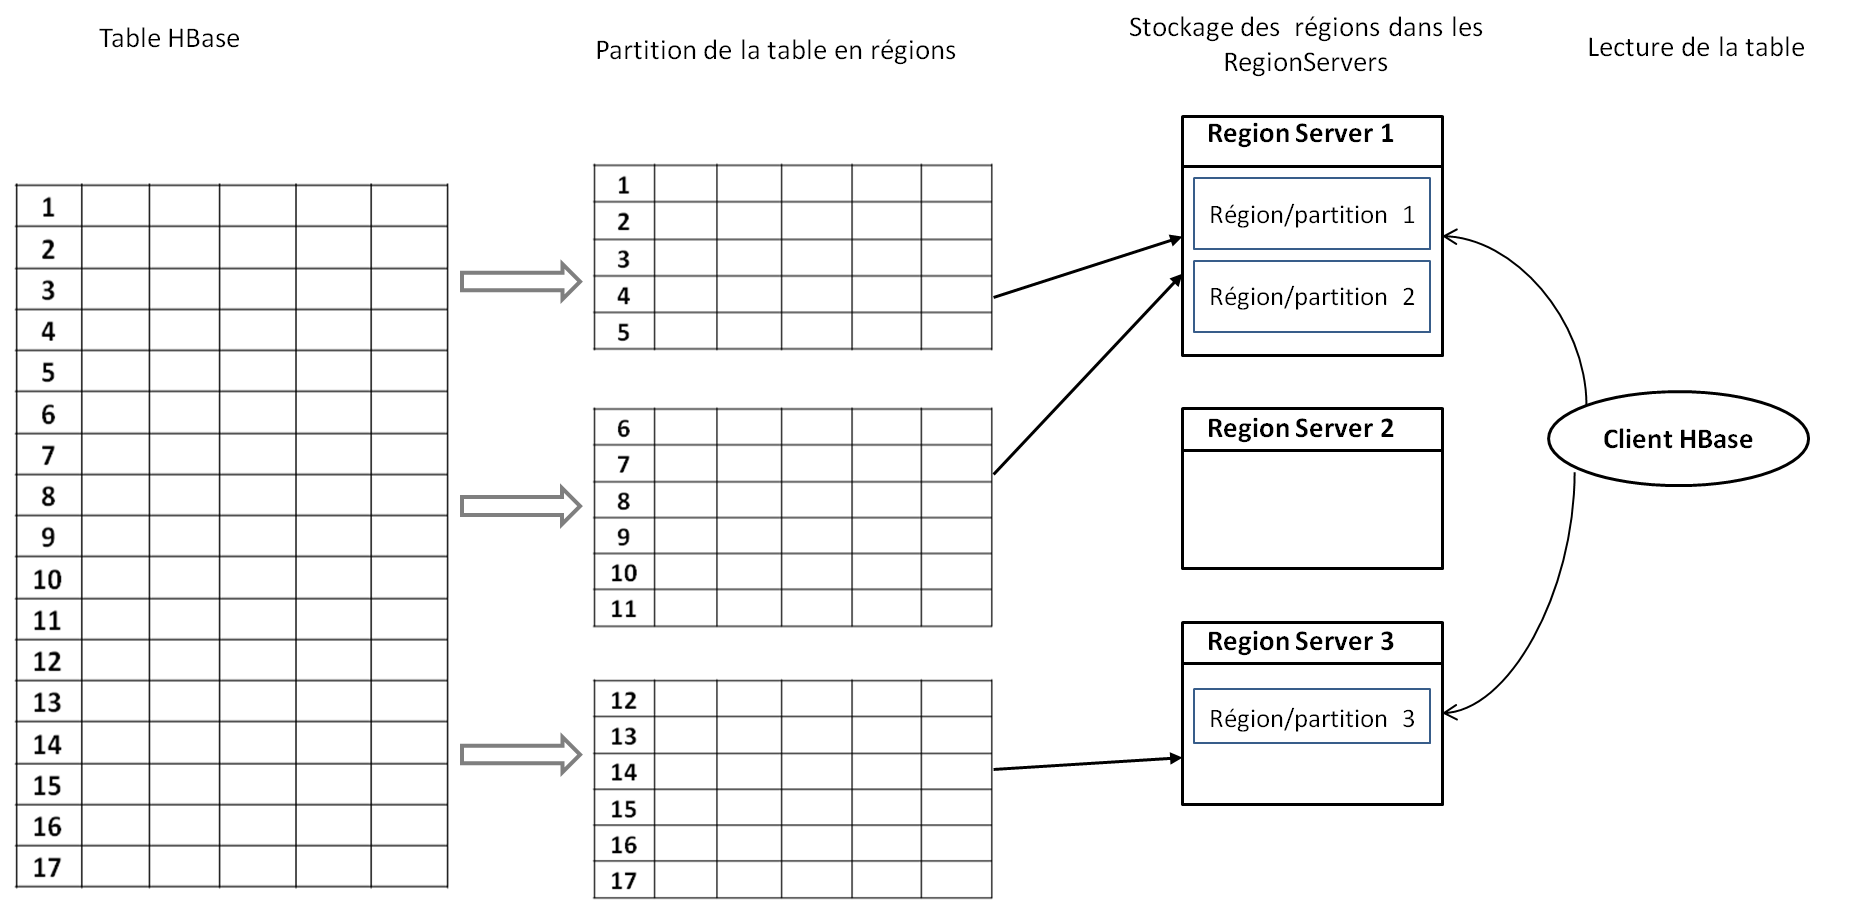
\includegraphics[scale=0.5]{img/part2/2.3}
    \caption{Architecture HBase.}
\end{figure}

\begin{enumerate}[label=\protect\ding{\value*}, start=182]

\item \textbf{RegionServer: } Le RegionServer est le point d'entrée pour l'accès a la donnée. C'est le serveur maitre ou les données sont stockées il gère d'une part plusieurs processus et d'autre part plusieurs composants :

\begin{figure}[h]
	\centering
    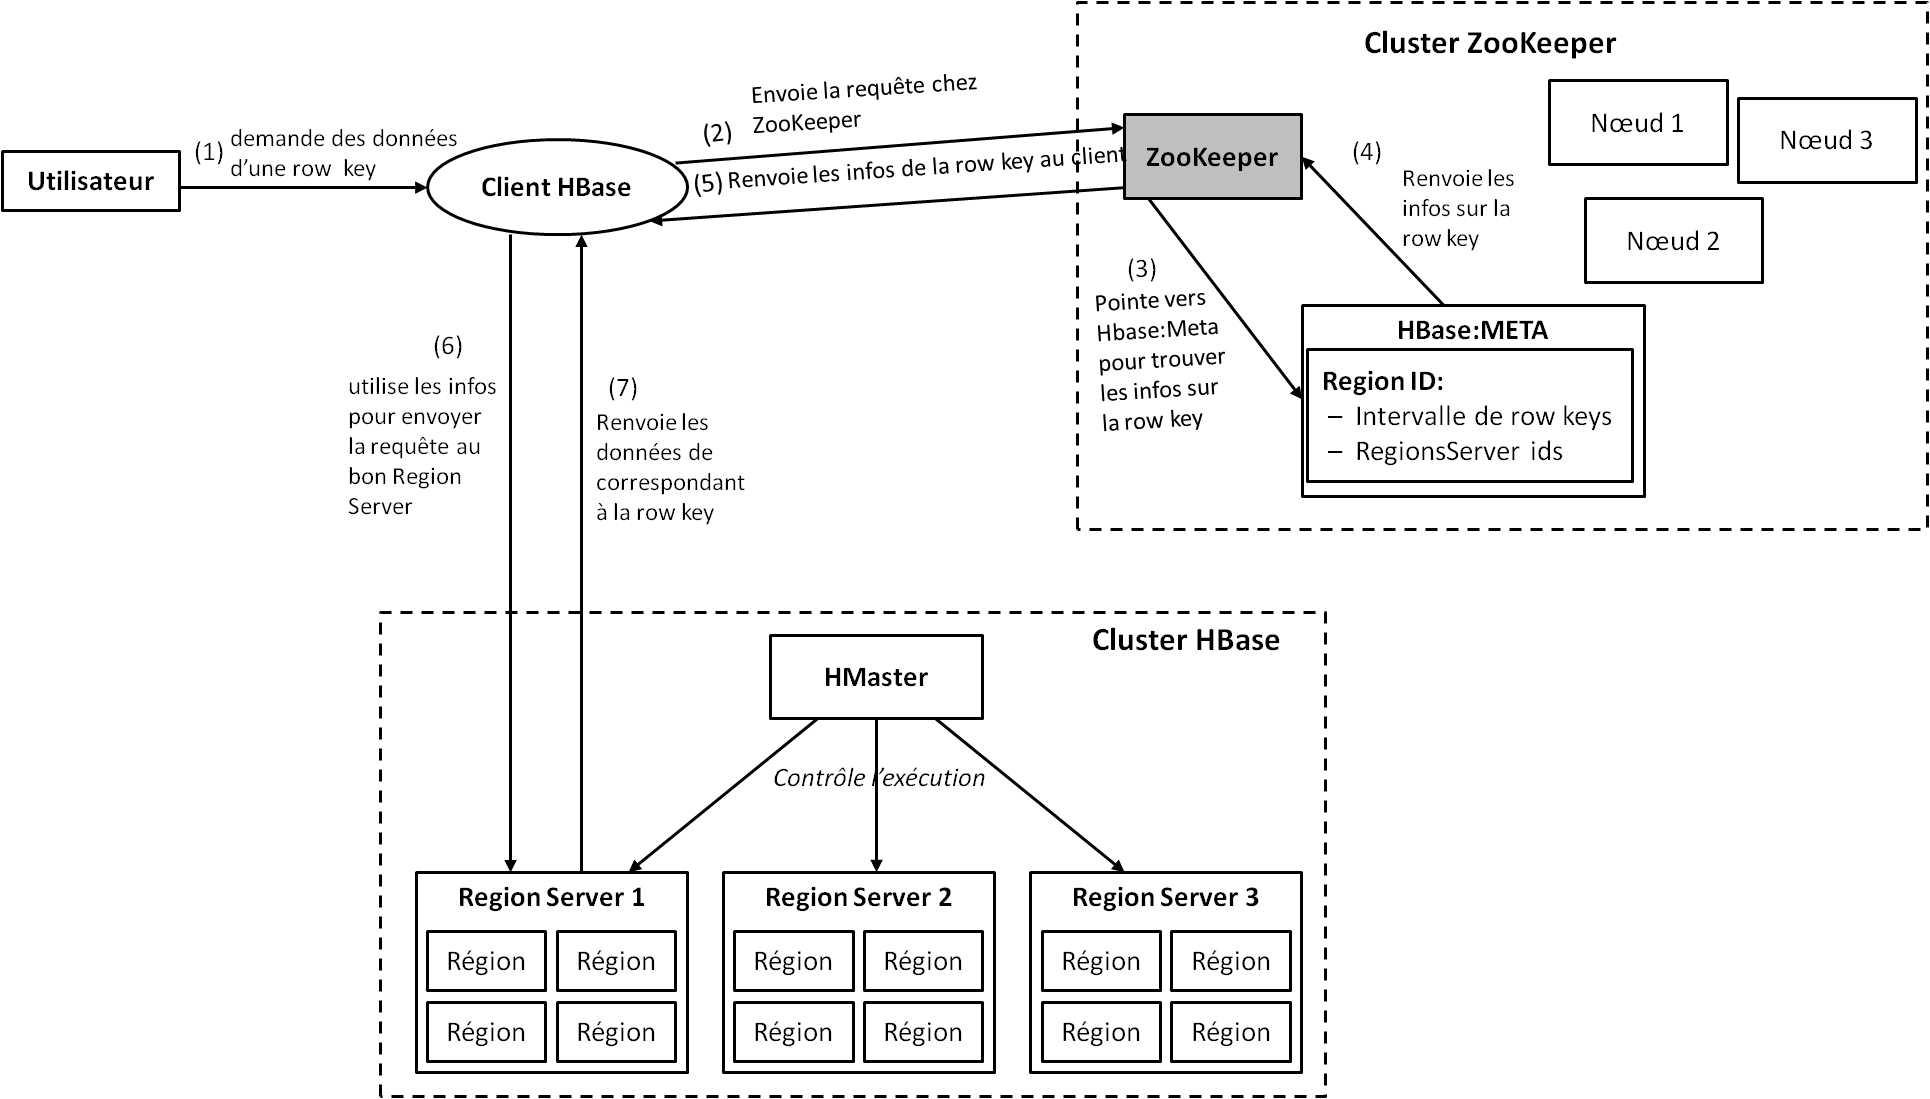
\includegraphics[scale=0.5]{img/part2/2.4}
    \caption{Anatomie de la base de données NoSQL HBase.}
\end{figure}

\item \textbf{La répartition des données :}
\begin{itemize}[label=\textbullet]
\item Les lignes d'une HTable sont scindées en paquets réguliers par le regionServer.
\item Chaque paquet est dirigé vers un serveur-esclave ou il est de nouveau divisé par le memstore selon les colonnes de la HTable.
\end{itemize}
		
\item \textbf{La gestion d'un WAL, un BlockCache et plusieurs Régions :}

\begin{itemize}[label=\textbullet]

\item  \textbf{BlockCache :} Le BlockCache est un cache LRU. Il est activé par défaut pour toutes les tables, ce qui signifie que toute opération de lecture sont chargées dans le cache LRU.

\item \textbf{Write Ahead Log (WAL) :} Chaque ajoute ou mises a jour dans un RegionServer sont systématiquement écrit dans write-ahead log (WAL) en premier lieu. Avant d'être répliquer dans le MemStore. Ce mécanisme garantit la durabilité de la donnée en cas de défaillance du serveur. Le processus WAL écrit dans le fichier Hlog qui est placé dans HDFS. Pour chaque instance. RegionServer il y a une instance de WAL.

\item \textbf{Region :} C'est l'élément de base dans le stockage et la distribution de la donnée dans HBase, dont l'implémentation est HRegion. Chaque Région gère un sous ensemble d'une table HBase (une partition). Une Région est composé de :
	\begin{itemize}
	\item \textit{Store :} Chaque partition d'une ColomnFamily est gérée par un store.
	HStore est l'implémentation d'un Store, il est compose de plusieurs StoreFiles
	et d'un MemStore.
	\item \textit{MemStore :} C'est un cache en mémoire. Il stocke toutes les écritures et les mises a 			jours relatives a une partition.
	\item \textit{Hfile}fichier physique sur lequel les données sont sauvegardées.
	\end{itemize}
	
	\begin{figure}[h]
	\centering
    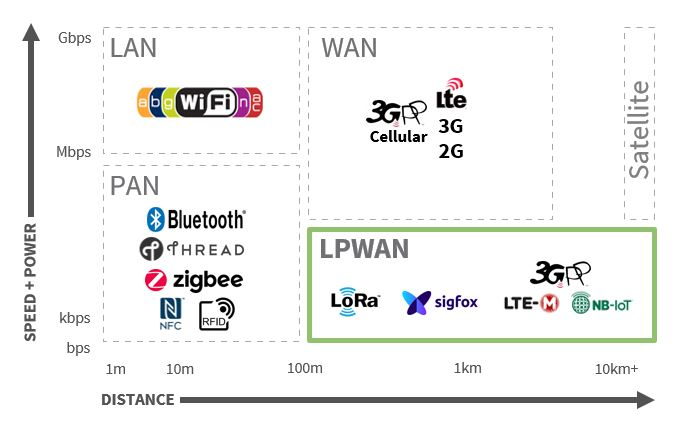
\includegraphics[scale=0.6]{img/part2/2.5}
    \caption{Récapitulatif du rôle de Région.}
	\end{figure}
\end{itemize}

\item \textbf{Zookeeper:}
Le projet open-source Apache ZooKeeper est un système open-source de synchronisation et de coordination des systèmes distribués, il permet de maintenir des informations de configuration. Il propose aussi des services synchronisés et des services de groupe pour une large variété d'applications distribuées. Cette technologie est déployée sur un cluster Hadoop pour administrer l'infrastructure. 

ZooKeeper facilite la synchronisation entre les process en maintenant un statut sur les serveurs ZooKeeper qui stocke l'information sur des fichiers de log locaux. Les serveurs ZooKeeper sont en mesure de supporter un large cluster Hadoop. Chaque machine client communique avec l'un des serveurs pour retrouve l'information.

\textbf{Exemple:} Soit un cluster Hadoop constitué de plus de 500 serveurs. Compte tenu du nombre de serveurs, une gestion centralisée du cluster s'impose pour les services de noms, de synchronisation ou pour la configuration et bien plus encore. En utilisant ZooKeeper, il est possible d'éviter d'avoir a développer des services de synchronisation en partant de zero. 

En effet il surveille l'état du cluster et informe régulièrement le MasterServer
des différents états. De plus, il stocke les informations critiques du cluster, dans l'emplacement de la table système -ROOT-.

\begin{itemize}
\item ROOT : contient la liste des tables .META. et leurs emplacements.
\item META : contient la liste des Régions et leurs emplacements.
\end{itemize}

\begin{figure}[h]
\centering
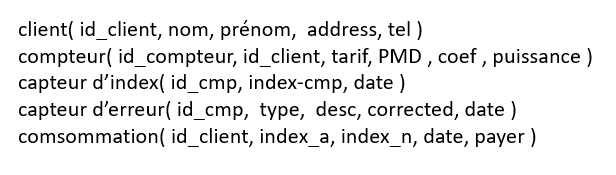
\includegraphics[scale=0.6]{img/part2/2.6}
\caption{Gestion des métadonnées avec ZooKeeper.}
\end{figure}

\end{enumerate}


\subsubsection*{3. MasterServer}
HMaster est l'implémentation du Master Server. Le Master Server est chargé de coordonner et de surveiller toutes les instances de RegionServer du cluster. Il en charge de la répétition des Région(s) sur les nœuds du cluster. Les changements dans les tables metadonnées passe par le serveur Master Server.

	




























